\subsection{Solar PV, utility scale (655~\$/kW)}\label{sec:solar-utility}
Utility-scale solar PV has seen extensive learning, and is the cheapest clean source of electricity in sunny regions.

The CAPEX of 655~\$/kW is the 2025 value of the Danish Energy Agency (DEA) catalogue \citep{dea} as carried by technology-data \citep{technologydata}.
We apply an exogenous cost path from the DEA projections \citep{dea}.
For reference, installed costs have fallen by about a third with each doubling of cumulative capacity (Figure~\ref{fig:solar}).

\begin{figure}[htbp]\centering
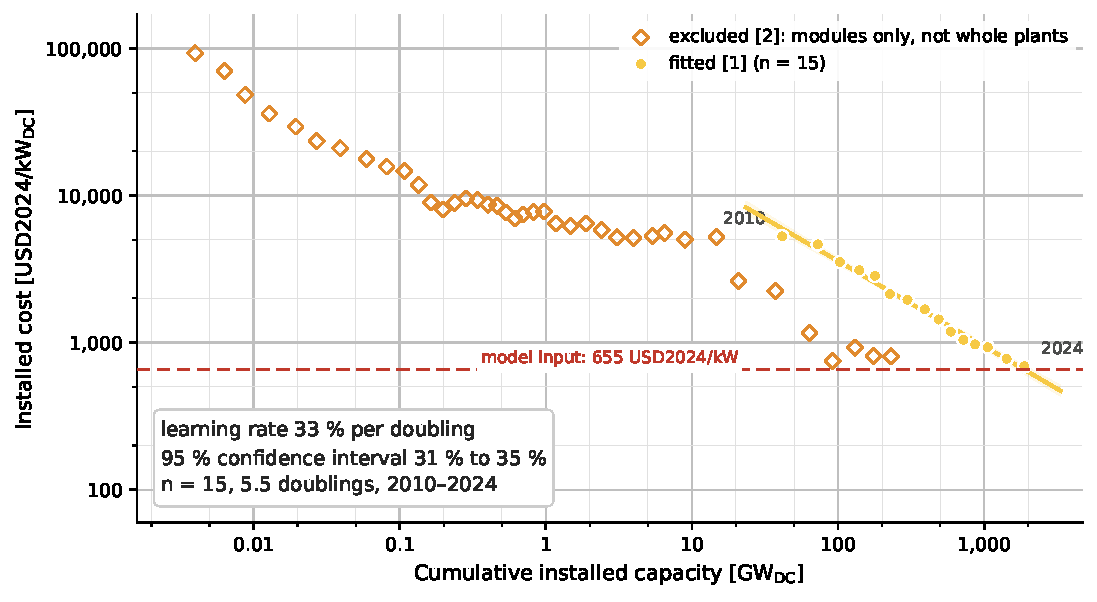
\includegraphics[width=\textwidth]{../../../misc-quarter1/technology-costs/figures/learning/solar-utility.pdf}
\caption{Installed cost of utility-scale PV against cumulative capacity.
Sources: [1] \citet{irena2025}, fitted; [2] module prices of \citet{schmidt2018}, for context.
Dashed red line: the model input.}\label{fig:solar}
\end{figure}

The fixed O\&M and the 37.5-year lifetime come from technology-data \citep{technologydata}, existing capacity from Ember \citep{ember2025}.
The capacity factor of 0.18 in Table~\ref{tab:costs} is a reference value, while the model uses hourly weather-based profiles for every region (Figure~\ref{fig:solar-maps}).

\begin{figure}[htbp]\centering
\begin{subfigure}[t]{0.49\textwidth}\centering
\includegraphics[width=\linewidth]{../build/figures/solar-utility_cf.pdf}
\caption{Annual mean capacity factor}
\end{subfigure}\hfill
\begin{subfigure}[t]{0.49\textwidth}\centering
\includegraphics[width=\linewidth]{../build/figures/solar-utility_lcoe.pdf}
\caption{Levelised cost of electricity}
\end{subfigure}
\caption{Utility-scale solar PV on land, 0.5$^\circ$ cells.
Left: annual mean capacity factor from ERA5 weather of 2011 \citep{hersbach2020}, as converted by \href{https://model.energy}{model.energy} \citep{modelenergy}.
Right: the levelised cost this implies with the costs of Table~\ref{tab:costs} at a 7\,\% real discount rate; colour scale logarithmic.}\label{fig:solar-maps}
\end{figure}

Regional differences in the cost of capital could be considered: in low- and middle-income countries, high financing costs add on average 26~\$/MWh to the levelised cost of solar \citep{hatton2026}.
